% Provenance (never printed): see sources/outline_sources.md (Year 1: internal
% structure of the Earth from seismology; reference model; density, gravity and
% pressure inside the Earth; mantle mineralogy; lithosphere and asthenosphere).
% Curves from figdata/bachelor-1/prem_profiles.py (shared dataset data:prem) and
% figdata/bachelor-1/refraction.py (generic two-layer crust); exercise and problem
% values in the Book 3 scratch calculator calc/ch09.py.
\chapter{The Layered Earth}\label{ch:b1:layered-earth}

On 8 October 1909 an earthquake shook the Kupa valley, south-east of Zagreb.
% ledger: skoko:mohorovicic
Andrija Mohorovičić, who ran the observatory there, gathered the seismograms
recorded across Europe and noticed something odd: up to a few hundred
kilometres from the epicentre the first tremor came in one way, farther out a
second kind of first arrival took over, as if part of the energy had found a
faster road at depth. He explained it by a boundary some fifty kilometres down,
below which the waves travel faster: the base of the \omterm{def:b1:layered-earth:layers}{crust}. A century of such
records, millions of them, has turned that first boundary into a reference
model of the whole Earth, layer by layer, with its velocities, its density, its
gravity and its pressure down to the centre. This chapter shows how a
boundary is found from travel times, what the reference model says, how a
density profile is drawn from seismic velocities alone and checked against the
Earth's mass and moment of inertia, which \omterm{def:b1:rock-forming-minerals:mineral}{minerals} make the \omterm{def:b1:layered-earth:layers}{mantle} at each
depth, what the core is made of, and where the rigid outer shell of the planet
ends.

\begin{recall}
A P wave is a compression wave, an S wave a shear wave; S waves do not cross
liquids, and the P and S shadow zones of the core give the radius of the liquid
\omterm{def:b1:layered-earth:layers}{outer core} (Book 2, grade 11). Waves are refracted at a boundary according to
Snell's law, $\sin i_1/v_1 = \sin i_2/v_2$ (physics). In a fluid at rest the
pressure grows with depth as $\mathrm dP = \rho g\,\mathrm dz$ (physics,
University Year 1). The \omterm{def:b1:layered-earth:layers}{crust}, the \omterm{def:b1:layered-earth:layers}{mantle} and the core were introduced in
Book 1 (grade 6).
\end{recall}

\section{Seismic waves in a layered Earth}

The speeds of seismic waves depend on the elastic moduli of the rock and on
its density. The physics books derive them from the equations of continuum
elasticity; here they are taken as known.

\begin{proposition}[Seismic speeds]\label{prop:b1:layered-earth:speeds}
In an isotropic elastic solid of density $\rho$, bulk modulus $K$ and shear
modulus $\mu$, P and S waves travel at
\[
  v_P = \sqrt{\frac{K + \tfrac43\mu}{\rho}}, \qquad v_S = \sqrt{\frac{\mu}{\rho}}.
\]
In a liquid $\mu = 0$: $v_S = 0$ and no S wave propagates.
\end{proposition}
\admitted

Since $K$ and $\mu$ are positive, $v_P > v_S$ always: in PREM's \omterm{def:b1:layered-earth:layers}{crust} and
\omterm{def:b1:layered-earth:layers}{mantle} $v_P$ is about $1.8$ to $1.9$ times $v_S$, and P waves arrive first. Both speeds
generally grow with depth, because pressure stiffens the rock more than it
compresses it, so that rays bend back towards the surface; and at a few depths
they jump.

\begin{definition}[Seismic discontinuity, Moho, core--mantle and inner-core boundaries]
\label{def:b1:layered-earth:discontinuity}
A \emph{seismic discontinuity}\index{seismic discontinuity} is a surface
inside the Earth across which the seismic speeds, the density or both change
abruptly, over a thickness small compared with a seismic wavelength. The
\emph{Mohorovičić discontinuity}\index{Mohorovičić discontinuity} (or
\emph{Moho}\index{Moho}) is the base of the \omterm{def:b1:layered-earth:layers}{crust}, where $v_P$ jumps to about
\qty{8}{km.s^{-1}}. The \emph{core--mantle boundary}\index{core--mantle
boundary} is the surface between the solid silicate \omterm{def:b1:layered-earth:layers}{mantle} and the liquid
\omterm{def:b1:layered-earth:layers}{outer core}; the \emph{inner-core boundary}\index{inner-core boundary} is the
surface between the liquid \omterm{def:b1:layered-earth:layers}{outer core} and the solid \omterm{def:b1:layered-earth:layers}{inner core}.
\end{definition}

\subsection{Refraction at a layer boundary}

Take a layer of thickness $h$ and speed $v_1$, the \omterm{def:b1:layered-earth:layers}{crust}, over a half-space of
speed $v_2 > v_1$, the \omterm{def:b1:layered-earth:layers}{mantle}, and a source at the surface. Three waves reach a
receiver at the distance $x$. The direct wave travels in the layer, at $v_1$.
The reflected wave bounces off the boundary. And a ray that strikes the
boundary at the critical angle $i_c$, with $\sin i_c = v_1/v_2$, is refracted
along it, travels in the faster medium just below it at the speed $v_2$, and
sends energy back up into the layer at the same angle $i_c$ all along its way.

\begin{definition}[Head wave, crossover distance]\label{def:b1:layered-earth:head-wave}
A \emph{head wave}\index{head wave} is the wave that travels along a boundary
at the speed of the faster medium below it and leaves it upward at the critical
angle. The \emph{crossover distance}\index{crossover distance} is the distance
from the source beyond which the head wave arrives before the direct wave.
\end{definition}

\begin{theorem}[Travel times over a two-layer Earth]\label{thm:b1:layered-earth:two-layer}
Over a layer of thickness $h$ and speed $v_1$ resting on a half-space of speed
$v_2 > v_1$, a surface source and a surface receiver at the distance $x$ give
\[
  t_{\text{direct}} = \frac{x}{v_1}, \qquad
  t_{\text{head}} = \frac{x}{v_2} + \frac{2h\cos i_c}{v_1}
  \quad (x \ge 2h\tan i_c), \qquad \sin i_c = \frac{v_1}{v_2},
\]
and the \omterm{def:b1:layered-earth:head-wave}{head wave} arrives first beyond the \omterm{def:b1:layered-earth:head-wave}{crossover distance}
\[
  x_c = 2h\sqrt{\frac{v_2 + v_1}{v_2 - v_1}}.
\]
\end{theorem}

\begin{proof}
The \omterm{def:b1:layered-earth:head-wave}{head wave} goes down at the angle $i_c$ through the layer, a path of length
$h/\cos i_c$, runs along the boundary over the distance $x - 2h\tan i_c$, and
comes up along a path of length $h/\cos i_c$. Its travel time is
\[
  t_{\text{head}} = \frac{2h}{v_1\cos i_c} + \frac{x - 2h\tan i_c}{v_2}
  = \frac{x}{v_2} + \frac{2h}{v_1\cos i_c}\Bigl(1 - \frac{v_1\sin i_c}{v_2}\Bigr)
  = \frac{x}{v_2} + \frac{2h}{v_1\cos i_c}\,(1 - \sin^2 i_c),
\]
that is $x/v_2 + 2h\cos i_c/v_1$. The path exists only if the horizontal run
is positive, $x \ge 2h\tan i_c$. The two times are equal when
$x(1/v_1 - 1/v_2) = 2h\cos i_c/v_1$; with $\cos i_c = \sqrt{v_2^2 - v_1^2}/v_2$,
\[
  x\,\frac{v_2 - v_1}{v_1 v_2} = \frac{2h\sqrt{(v_2 - v_1)(v_2 + v_1)}}{v_1 v_2},
\]
which gives $x_c$. Beyond it the head-wave line, of smaller slope $1/v_2$,
lies below the direct-wave line.
\end{proof}

On a plot of travel time against distance, the direct and \omterm{def:b1:layered-earth:head-wave}{head waves} are two
straight lines. Their slopes are the inverse speeds $1/v_1$ and $1/v_2$; the
head-wave line, extended back to $x = 0$, cuts the time axis at the
\emph{intercept time} $t_i = 2h\cos i_c/v_1$. The reflected wave,
$t = \sqrt{x^2 + 4h^2}/v_1$, is a hyperbola that touches the head-wave line at
the critical distance $2h\tan i_c$, where the \omterm{def:b1:layered-earth:head-wave}{head wave} is born (\cref{exo:b1:layered-earth:10}).

\begin{omfigure}
\begin{tabular}{@{}c@{}}
\begin{tikzpicture}
\begin{axis}[width=0.86\linewidth, axis equal image, xmin=0, xmax=260, ymin=-62, ymax=8,
  axis x line=top, axis y line=left, axis line style={-}, clip=false,
  ylabel={depth (km)}, ytick={-60,-35,0},
  yticklabels={60,35,0}, tick label style={font=\scriptsize}, label style={font=\small}]
\fill[brown!12] (axis cs:0,0) rectangle (axis cs:260,-35);
\fill[orange!18] (axis cs:0,-35) rectangle (axis cs:260,-62);
\draw[black!60] (axis cs:0,-35) -- (axis cs:260,-35);
\addplot[very thick, blue!70!black] table[x=x, y=z, unbounded coords=jump,
  restrict expr to domain={\coordindex}{0:1}] {figdata/out/bachelor-1-refraction-rays.dat};
\addplot[thick, dashed, green!45!black] table[x=x, y=z, unbounded coords=jump,
  restrict expr to domain={\coordindex}{3:5}] {figdata/out/bachelor-1-refraction-rays.dat};
\addplot[very thick, red!75!black] table[x=x, y=z, unbounded coords=jump,
  restrict expr to domain={\coordindex}{7:10}] {figdata/out/bachelor-1-refraction-rays.dat};
\node[font=\scriptsize, anchor=north west] at (axis cs:2,-36) {mantle, $v_2 = \qty{8.0}{km.s^{-1}}$};
\node[font=\scriptsize, anchor=center] at (axis cs:125,-17) {crust, $v_1 = \qty{6.0}{km.s^{-1}}$, $h = \qty{35}{km}$};
\node[font=\scriptsize, red!75!black, anchor=north] at (axis cs:150,-36) {head wave along the Moho};
\node[font=\scriptsize, green!45!black, anchor=south] at (axis cs:40,-20) {reflected};
\node[font=\scriptsize, blue!70!black, anchor=north] at (axis cs:125,-1) {direct};
\fill (axis cs:0,0) circle (2pt);
\end{axis}
\end{tikzpicture}\\[2pt]
{\small (a) ray paths (distance in km)}\\[6pt]
\begin{tikzpicture}
\begin{axis}[omrecord, width=0.86\linewidth, height=6.0cm, xmin=0, xmax=400, ymin=0, ymax=70,
  xlabel={distance $x$ (km)}, ylabel={travel time $t$ (s)}, tick label style={font=\scriptsize},
  label style={font=\small}, clip=false,
  legend style={font=\scriptsize, at={(0.03,0.97)}, anchor=north west, draw=none, fill=white, fill opacity=0.85}]
\addplot[very thick, blue!70!black] table[x=x, y=t_direct] {figdata/out/bachelor-1-refraction-times.dat};
\addlegendentry{direct, slope $1/v_1$}
\addplot[thick, dashed, green!45!black] table[x=x, y=t_reflected] {figdata/out/bachelor-1-refraction-times.dat};
\addlegendentry{reflected}
\addplot[very thick, red!75!black, unbounded coords=jump] table[x=x, y=t_head] {figdata/out/bachelor-1-refraction-times.dat};
\addlegendentry{head wave, slope $1/v_2$}
\addplot[thin, dotted, red!75!black, domain=0:79.37] {x/8 + 7.717};
\draw[black!60, densely dashed] (axis cs:185.2,0) -- (axis cs:185.2,30.87);
\node[font=\scriptsize, anchor=north west] at (axis cs:187,8) {$x_c = \qty{185}{km}$};
\node[font=\scriptsize, anchor=east, red!75!black] at (axis cs:-3,7.7) {$t_i$};
\end{axis}
\end{tikzpicture}\\[2pt]
{\small (b) travel times}
\end{tabular}

\par\smallskip{\small Refraction over a \omterm{def:b1:layered-earth:layers}{crust} \qty{35}{km} thick, at \qty{6.0}{km.s^{-1}},
on a \omterm{def:b1:layered-earth:layers}{mantle} at \qty{8.0}{km.s^{-1}} ((a) at true scale). (a) The direct wave runs along the surface; the reflected wave
drawn is the one that strikes the Moho at the critical angle,
\ang{48.6}; the \omterm{def:b1:layered-earth:head-wave}{head wave} runs along the \omterm{def:b1:layered-earth:discontinuity}{Moho} and returns at that angle. (b)
Arrival times: the \omterm{def:b1:layered-earth:head-wave}{head wave} appears at the critical distance,
\qty{79}{km}, tangent to the reflection, and overtakes the direct wave at the
\omterm{def:b1:layered-earth:head-wave}{crossover distance}, \qty{185}{km}. The dotted extension gives the intercept
time $t_i = \qty{7.7}{s}$.}
\end{omfigure}

\begin{method}[The depth of a boundary from a refraction profile]\label{met:b1:layered-earth:moho}
\begin{enumerate}
  \item Plot the first-arrival times against distance, and fit one straight
        line through the arrivals close to the source and another through the
        distant ones.
  \item The inverse slopes give $v_1$ and $v_2$; then $\sin i_c = v_1/v_2$.
  \item Read the intercept time $t_i$ of the distant line at $x = 0$, and
        compute $h = t_i v_1/(2\cos i_c)$; check it with the \omterm{def:b1:layered-earth:head-wave}{crossover
        distance}, $h = \tfrac12 x_c\sqrt{(v_2 - v_1)/(v_2 + v_1)}$.
  \item A boundary is found only if $v_2 > v_1$: a slower layer below a faster
        one produces no \omterm{def:b1:layered-earth:head-wave}{head wave} and stays hidden.
\end{enumerate}
\end{method}

Mohorovičić's two kinds of first arrival were exactly these two lines: the
direct wave in the \omterm{def:b1:layered-earth:layers}{crust} near the source, the \omterm{def:b1:layered-earth:head-wave}{head wave} along the top of the
\omterm{def:b1:layered-earth:layers}{mantle} farther out. His figure for the thickness of the \omterm{def:b1:layered-earth:layers}{crust} in that region,
\qty{54}{km}, has been confirmed in its order of size, but the depth of the \omterm{def:b1:layered-earth:discontinuity}{Moho}
varies from place to place. Under the oceans the \omterm{def:b1:layered-earth:layers}{crust} is only about
\qty{5}{km} thick; under the continents it averages about \qty{30}{km}, and it
is much thicker under large mountain ranges. For its reference model, PREM took
the \omterm{def:b1:layered-earth:discontinuity}{Moho} at \qty{11}{km} below sea level under the oceans and \qty{35}{km} under
the continents.
% ledger: skoko:mohorovicic, usgs:crust-thickness, prem:moho-average

\begin{history}[Andrija Mohorovičić]
\begin{minipage}[t]{0.76\linewidth}\vspace{0pt}
% ledger: skoko:mohorovicic
Andrija Mohorovičić (1857--1936) came to seismology from meteorology: a
teacher, then from 1891 to 1921 the director of the meteorological observatory
of Zagreb, he published his last meteorological study in 1901. On the
seismograms of the Kupa valley earthquake of 8 October 1909 he found two
distinct pairs of P and S phases: near the source one kind of first tremor
arrived first, farther away another, which had travelled faster at depth. His
reading of these two arrivals as a
direct wave and a wave refracted below a boundary gave the boundary that now
bears his name, and the first measure of the thickness of the \omterm{def:b1:layered-earth:layers}{crust}.
\end{minipage}\hfill
\begin{minipage}[t]{0.2\linewidth}\vspace{0pt}
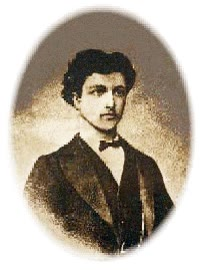
\includegraphics[width=\linewidth]{images/book3/b1-mohorovicic.jpg}

{\scriptsize Andrija Mohorovičić. Public domain.}
\end{minipage}
\end{history}

\section{A reference Earth model}

The same reasoning, applied to millions of travel times at all distances and
to the periods of the Earth's free oscillations (the whole planet rings like a
bell after a large earthquake), gives the speeds at every depth.

\begin{definition}[Reference Earth model]\label{def:b1:layered-earth:reference-model}
A \emph{reference Earth model}\index{reference Earth model} is a
spherically symmetric Earth, given as the seismic speeds $v_P(r)$, $v_S(r)$,
the density $\rho(r)$ and, in the fullest models, the attenuation as functions
of the radius $r$ alone, that fits the observed travel times, free-oscillation
periods, the Earth's mass and its moment of inertia. The most widely used is
PREM, the Preliminary Reference Earth Model (1981).
\end{definition}

PREM was fitted to the radius \qty{6371}{km}, the mass
\qty{5.974e24}{kg} and the \omterm{def:b1:comparative-planetology:moi}{moment-of-inertia factor} $0.3308$ of the Earth.
It divides the planet into a few regions joined by discontinuities, and its
profiles (figure below) show at once the main layers.

\begin{definition}[Crust, mantle, outer core, inner core]\label{def:b1:layered-earth:layers}
The \emph{crust}\index{crust} is the outer silicate layer above the \omterm{def:b1:layered-earth:discontinuity}{Moho}. The
\emph{mantle}\index{mantle} is the solid silicate shell between the \omterm{def:b1:layered-earth:discontinuity}{Moho} and
the \omterm{def:b1:layered-earth:discontinuity}{core--mantle boundary}, at a depth of about \qty{2891}{km}. The
\emph{outer core}\index{outer core} is the liquid metallic shell between the
\omterm{def:b1:layered-earth:discontinuity}{core--mantle boundary} and the \omterm{def:b1:layered-earth:discontinuity}{inner-core boundary}, at about \qty{5150}{km}
depth. The \emph{inner core}\index{inner core} is the solid metallic sphere
below it, of radius about \qty{1220}{km}.
\end{definition}

\begin{omfigure}
\begin{tikzpicture}
\begin{axis}[omrecord, omdepth, width=0.62\linewidth, height=5.4cm, xmin=0, xmax=14, ymin=0, ymax=6371,
  xlabel={speed (\unit{km.s^{-1}}) or density (\unit{g.cm^{-3}})}, ylabel={depth (km)},
  ytick={0,1000,...,6000}, tick label style={font=\scriptsize}, label style={font=\small},
  clip=false, legend style={font=\scriptsize, at={(0.02,0.80)}, anchor=north west, draw=none, fill=white}]
\addplot[very thick, blue!70!black] table[x=vp, y=depth] {figdata/out/bachelor-1-prem_profiles-profiles.dat};
\addlegendentry{$v_P$}
\addplot[very thick, red!75!black] table[x=vs, y=depth] {figdata/out/bachelor-1-prem_profiles-profiles.dat};
\addlegendentry{$v_S$}
\addplot[very thick, black!70, densely dashed] table[x=rho, y=depth] {figdata/out/bachelor-1-prem_profiles-profiles.dat};
\addlegendentry{$\rho$}
\draw[black!35] (axis cs:0,670) -- (axis cs:14,670) node[right, font=\scriptsize, black] {670 km};
\draw[black!35] (axis cs:0,2891) -- (axis cs:14,2891) node[right, font=\scriptsize, black] {core--mantle boundary};
\draw[black!35] (axis cs:0,5149.5) -- (axis cs:14,5149.5) node[right, font=\scriptsize, black] {inner-core boundary};
\node[font=\scriptsize, anchor=west] at (axis cs:14,1700) {mantle};
\node[font=\scriptsize, anchor=west] at (axis cs:14,4000) {outer core (liquid)};
\node[font=\scriptsize, anchor=west] at (axis cs:14,5800) {inner core (solid)};
\end{axis}
\end{tikzpicture}

\par\smallskip{\small PREM: the speeds of P and S waves and the density against depth.
The S speed falls to zero in the liquid \omterm{def:b1:layered-earth:layers}{outer core} and reappears, small, in the
solid \omterm{def:b1:layered-earth:layers}{inner core}; at the \omterm{def:b1:layered-earth:discontinuity}{core--mantle boundary} the density almost doubles
while $v_P$ drops from 13.7 to \qty{8.1}{km.s^{-1}}; the jumps near
\qty{400}{km} and \qty{670}{km} bound the transition zone.}
\end{omfigure}

\begin{table}[htbp]
\centering
\footnotesize
\setlength{\tabcolsep}{3pt}
\begin{tabular}{>{\raggedright\arraybackslash}p{0.2\linewidth}rr>{\raggedright\arraybackslash}p{0.47\linewidth}}
\hline
boundary in PREM & depth (km) & radius (km) & what changes \\
\hline
\omterm{def:b1:layered-earth:discontinuity}{Moho} & 24.4 & 6346.6 & \omterm{def:b1:layered-earth:layers}{crust} above, peridotite below; $v_P$ 6.8 to 8.1 \\
220-km discontinuity & 220 & 6151 & base of the \omterm{def:b1:layered-earth:lithosphere}{low-velocity zone} in PREM \\
400-km discontinuity & 400 & 5971 & \omterm{def:b1:rock-forming-minerals:groups}{olivine} to wadsleyite (\qty{410}{km} in most studies) \\
670-km discontinuity & 670 & 5701 & ringwoodite to bridgmanite and ferropericlase (\qty{660}{km} in most studies) \\
\omterm{def:b1:layered-earth:discontinuity}{core--mantle boundary} & 2891 & 3480 & silicate to liquid iron; $v_S$ 7.3 to 0; $\rho$ 5.57 to 9.90 \\
\omterm{def:b1:layered-earth:discontinuity}{inner-core boundary} & 5149.5 & 1221.5 & liquid to solid iron; $v_S$ 0 to 3.5; $\rho$ 12.17 to 12.76 \\
\hline
\end{tabular}
\caption{The main discontinuities of PREM (speeds in \unit{km.s^{-1}}, densities
in \unit{g.cm^{-3}}). PREM averages the \omterm{def:b1:layered-earth:layers}{crust} to \qty{24.4}{km}; real \omterm{def:b1:layered-earth:layers}{crusts}
range from about \qty{5}{km} under the oceans to many tens of kilometres under
mountain ranges.}
% ledger: usgs:crust-thickness
\label{tab:b1:layered-earth:prem}
\end{table}

Two facts in these profiles are directly observed. The vanishing of $v_S$ in
the \omterm{def:b1:layered-earth:layers}{outer core} is the S-wave shadow recalled above: S waves enter the core only
as P waves, the core cannot transmit shear, so it is liquid. And the \omterm{def:b1:layered-earth:layers}{inner core}
transmits S waves, slowly: it is solid. That second fact came from weak P
arrivals where no P wave should be.

\begin{history}[Inge Lehmann and the inner core]
% ledger: hjortenberg:lehmann
\begin{minipage}[t]{0.76\linewidth}\vspace{0pt}
Inge Lehmann (1888--1993), head of the seismological department of the
Danish geodetic institute, studied the records of the 1929 Buller
earthquake in New Zealand and found P waves arriving inside the shadow zone,
where the core should have bent them away. In a paper of 1936 with the
shortest of titles, \emph{P$'$}, she showed that they could be explained if the
core held a smaller \omterm{def:b1:layered-earth:layers}{inner core} with a higher P speed, which returns part of the
energy towards the surface. Her \omterm{def:b1:layered-earth:layers}{inner core} is now known to be solid, and to
grow slowly as the Earth cools. She also discovered the discontinuity
near \qty{220}{km} that bears her name.
\end{minipage}\hfill
\begin{minipage}[t]{0.2\linewidth}\vspace{0pt}
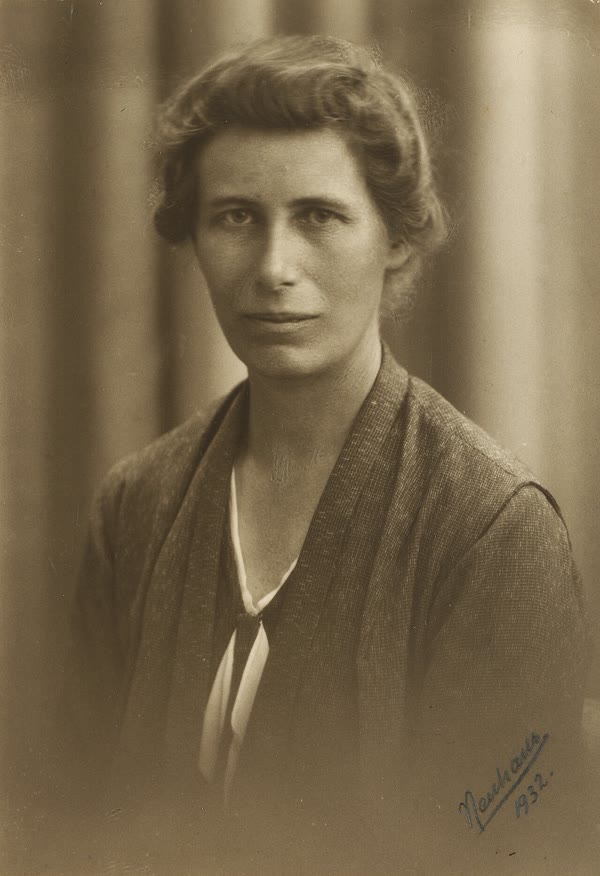
\includegraphics[width=\linewidth]{images/book3/b1-lehmann.jpg}

{\scriptsize Inge Lehmann in 1932, by Even Neuhaus. Public domain.}
\end{minipage}
\end{history}

\section{Density, gravity and pressure from seismic data}

Seismic speeds give two combinations of the moduli and the density, not the
density itself. A third relation comes from the assumption that, inside a
layer of uniform composition, the rock is simply compressed by the weight of
the rock above.

\begin{definition}[Seismic parameter]\label{def:b1:layered-earth:seismic-parameter}
The \emph{seismic parameter}\index{seismic parameter} at a depth is
\[
  \Phi = v_P^2 - \tfrac43 v_S^2 = \frac{K}{\rho},
\]
the bulk modulus divided by the density, computed from the two seismic speeds
alone (\cref{prop:b1:layered-earth:speeds}).
\end{definition}

\begin{theorem}[Adams--Williamson equation]\label{thm:b1:layered-earth:adams-williamson}
In a region of uniform composition, in hydrostatic equilibrium, compressed
adiabatically, the density varies with the radius as
\[
  \frac{\mathrm d\rho}{\mathrm dr} = -\frac{\rho(r)\,g(r)}{\Phi(r)},
\]
where $g(r)$ is the gravity at the radius $r$.
\end{theorem}

\begin{proof}
Hydrostatic equilibrium gives $\mathrm dP/\mathrm dr = -\rho g$ (the recall,
with $\mathrm dz = -\mathrm dr$). The bulk modulus is defined by
$K = \rho\,\mathrm dP/\mathrm d\rho$ for the compression at hand; for a rock of
fixed composition compressed without exchange of heat, it is the adiabatic
modulus that the seismic waves measure, so $\mathrm d\rho/\mathrm dP = \rho/K$.
By the chain rule,
\[
  \frac{\mathrm d\rho}{\mathrm dr} = \frac{\mathrm d\rho}{\mathrm dP}\,
  \frac{\mathrm dP}{\mathrm dr} = \frac{\rho}{K}\,(-\rho g) = -\frac{\rho g}{K/\rho}
  = -\frac{\rho g}{\Phi}. \qedhere
\]
\end{proof}

The equation fails at a discontinuity, where the composition or the crystal
structure changes, and wherever the temperature departs from the adiabat; but
between the discontinuities it accounts for the observed increase of density
with depth very well (panel (c) of the figure below). Starting from a density at the top of each
region, integrating it downward, and adjusting the starting values until the
mass and the moment of inertia come out right, is how the first density models
were built. The two global numbers are integrals of the density.

\begin{proposition}[Mass, gravity, pressure and moment of inertia]
\label{prop:b1:layered-earth:integrals}
For a spherically symmetric Earth of radius $R$ and density $\rho(r)$, the mass
inside the radius $r$, the gravity, the pressure and the moment of inertia
about an axis through the centre are
\[
  m(r) = \int_0^r 4\pi s^2\rho(s)\,\mathrm ds, \quad
  g(r) = \frac{G\,m(r)}{r^2}, \quad
  P(r) = \int_r^R \rho(s)\,g(s)\,\mathrm ds, \quad
  I = \frac{8\pi}{3}\int_0^R \rho(r)\,r^4\,\mathrm dr.
\]
\end{proposition}

\begin{proof}
A thin shell of radius $s$ and thickness $\mathrm ds$ has the volume
$4\pi s^2\,\mathrm ds$, hence the first integral. The gravity of a spherically
symmetric body outside a radius is that of its mass inside, concentrated at the
centre, and the shells outside $r$ pull with no net force (the shell theorem,
admitted from the physics books); hence $g(r)$. Integrating the hydrostatic
equation from the surface, where $P = 0$, gives $P(r)$. For the moment of
inertia, a thin spherical shell of mass $\mathrm dm$ and radius $r$ has, about
the three axes $x$, $y$, $z$, moments whose sum is
$\int (y^2 + z^2) + (z^2 + x^2) + (x^2 + y^2)\,\mathrm dm = 2r^2\,\mathrm dm$;
by symmetry the three are equal, so each is $\tfrac23 r^2\,\mathrm dm$. With
$\mathrm dm = 4\pi r^2\rho\,\mathrm dr$, summing the shells gives $I$.
\end{proof}

For a sphere of uniform density, $I = \tfrac{8\pi}{15}\rho R^5 = 0.4\,MR^2$.
The Earth's factor $I/MR^2 = 0.3308$ is smaller: its mass is concentrated
towards the centre, which is the first argument for a dense core. Computed from
PREM's density alone, the integrals give a mass of \qty{5.976e24}{kg}
(\qty{0.06}{\percent} above the measured \qty{5.972e24}{kg}), a factor $0.3309$,
and a central pressure of \qty{364}{GPa}, the value tabulated with PREM to
\qty{0.1}{\percent}.

\begin{omfigure}
\begin{tabular}{@{}c@{\hspace{2mm}}c@{\hspace{2mm}}c@{}}
\begin{tikzpicture}
\begin{axis}[omrecord, omdepth, width=0.35\linewidth, height=7.0cm, xmin=0, xmax=12, ymin=0, ymax=6371,
  xlabel={$g$ (\unit{m.s^{-2}})}, ylabel={depth (km)}, ytick={0,1000,...,6000}, xtick={0,4,8,12},
  tick label style={font=\scriptsize}, label style={font=\small}]
\addplot[very thick, blue!70!black] table[x=g, y=depth] {figdata/out/bachelor-1-prem_profiles-functionals.dat};
\draw[black!35] (axis cs:0,2891) -- (axis cs:12,2891);
\draw[black!35] (axis cs:0,5149.5) -- (axis cs:12,5149.5);
\node[font=\scriptsize, anchor=south west] at (axis cs:0.3,2891) {CMB};
\node[font=\scriptsize, anchor=south west] at (axis cs:0.3,5149.5) {ICB};
\end{axis}
\end{tikzpicture}
&
\begin{tikzpicture}
\begin{axis}[omrecord, omdepth, width=0.35\linewidth, height=7.0cm, xmin=0, xmax=400, ymin=0, ymax=6371,
  xlabel={$P$ (GPa)}, ytick={0,1000,...,6000}, yticklabels={}, xtick={0,200,400},
  tick label style={font=\scriptsize}, label style={font=\small}]
\addplot[very thick, red!75!black] table[x=P, y=depth] {figdata/out/bachelor-1-prem_profiles-functionals.dat};
\draw[black!35] (axis cs:0,2891) -- (axis cs:400,2891);
\draw[black!35] (axis cs:0,5149.5) -- (axis cs:400,5149.5);
\node[font=\scriptsize, anchor=south west] at (axis cs:150,2891) {\qty{136}{GPa}};
\node[font=\scriptsize, anchor=south east] at (axis cs:290,5149.5) {\qty{329}{GPa}};
\end{axis}
\end{tikzpicture}
&
\begin{tikzpicture}
\begin{axis}[omrecord, omdepth, width=0.35\linewidth, height=7.0cm, xmin=2, xmax=14, ymin=0, ymax=6371,
  xlabel={$\rho$ (\unit{g.cm^{-3}})}, ytick={0,1000,...,6000}, yticklabels={}, xtick={2,6,10,14},
  tick label style={font=\scriptsize}, label style={font=\small},
  legend style={font=\scriptsize, at={(0.97,0.97)}, anchor=north east, draw=none, fill=white}]
\addplot[very thick, black!55] table[x=rho, y=depth] {figdata/out/bachelor-1-prem_profiles-profiles.dat};
\addlegendentry{PREM}
\addplot[only marks, mark=o, mark size=1.4pt, orange!85!black, each nth point=15, unbounded coords=discard]
  table[x=rho_aw, y=depth] {figdata/out/bachelor-1-prem_profiles-adams.dat};
\addlegendentry{Adams--Williamson}
\end{axis}
\end{tikzpicture}
\\[2pt]
{\small (a) gravity} & {\small (b) pressure} & {\small (c) self-compression}
\end{tabular}

\par\smallskip{\small Inside the Earth, from PREM. (a) and (b) Gravity and pressure
computed from PREM's density with \cref{prop:b1:layered-earth:integrals}: gravity
stays close to \qty{10}{m.s^{-2}} through the \omterm{def:b1:layered-earth:layers}{mantle}, peaks at
\qty{10.7}{m.s^{-2}} at the \omterm{def:b1:layered-earth:discontinuity}{core--mantle boundary} (CMB) and falls to zero at the
centre; the pressure reaches \qty{136}{GPa} at the CMB, \qty{329}{GPa} at the
\omterm{def:b1:layered-earth:discontinuity}{inner-core boundary} (ICB) and \qty{364}{GPa} at the centre. (c) The
Adams--Williamson equation, integrated downward from PREM's density at
\qty{771}{km} and at the top of the \omterm{def:b1:layered-earth:layers}{outer core} with PREM's speeds and gravity
(circles), follows PREM to within \qty{0.2}{\percent}: there the density
increase is compression of a uniform material; the jumps are not.}
\end{omfigure}

That gravity grows on the way down through the \omterm{def:b1:layered-earth:layers}{mantle} is a direct consequence
of the dense core: the mass left inside the radius falls more slowly than
$r^2$. Through the \omterm{def:b1:layered-earth:layers}{mantle} $g$ hardly changes, and the pressure grows almost
linearly with depth, by about \qty{4.7}{GPa} per hundred kilometres.


\section{The mantle: one rock, several mineral assemblages}

The upper \omterm{def:b1:layered-earth:layers}{mantle} is peridotite, known from the fragments that volcanoes bring
up and from slices of \omterm{def:b1:layered-earth:layers}{mantle} thrust onto continents: about half to
three fifths \omterm{def:b1:rock-forming-minerals:groups}{olivine} by volume (\qtyrange{49}{62}{\percent} in the proposed
compositions), the rest \omterm{def:b1:rock-forming-minerals:groups}{pyroxenes} and an aluminous \omterm{def:b1:rock-forming-minerals:mineral}{mineral} (\omterm{def:b1:rock-forming-minerals:groups}{plagioclase},
spinel or \omterm{def:b1:rock-forming-minerals:groups}{garnet}, depending on depth). The pressure that rises with depth
does not change this composition, but it forces its atoms into denser
arrangements: \omterm{def:b1:rock-forming-minerals:polymorph}{polymorphs} (\cref{ch:b1:rock-forming-minerals}) appear one after
the other.

\begin{definition}[Mantle transition zone]\label{def:b1:layered-earth:transition-zone}
The \emph{mantle transition zone}\index{mantle transition zone} is the part
of the \omterm{def:b1:layered-earth:layers}{mantle} between the seismic discontinuities near \qty{410}{km} and
\qty{660}{km} depth, in which \omterm{def:b1:rock-forming-minerals:groups}{olivine} of the upper \omterm{def:b1:layered-earth:layers}{mantle} is replaced by its
denser \omterm{def:b1:rock-forming-minerals:polymorph}{polymorphs}, wadsleyite and then ringwoodite. Above it is the upper
\omterm{def:b1:layered-earth:layers}{mantle}; below it the lower \omterm{def:b1:layered-earth:layers}{mantle}, down to the \omterm{def:b1:layered-earth:discontinuity}{core--mantle boundary}.
\end{definition}

At about \qty{410}{km} (\qty{14}{GPa}) \omterm{def:b1:rock-forming-minerals:groups}{olivine} \ce{(Mg,Fe)2SiO4} becomes
wadsleyite, of the same formula; near \qty{520}{km} (\qty{17.5}{GPa}) wadsleyite
becomes ringwoodite; the \omterm{def:b1:rock-forming-minerals:groups}{pyroxenes} dissolve into a \omterm{def:b1:rock-forming-minerals:groups}{garnet} rich in silicon,
majorite, until by the middle of the transition zone \omterm{def:b1:rock-forming-minerals:groups}{garnet} holds all of them,
so that the zone is a little more than half \omterm{def:b1:rock-forming-minerals:groups}{olivine} \omterm{def:b1:rock-forming-minerals:polymorph}{polymorphs} and the rest
\omterm{def:b1:rock-forming-minerals:groups}{garnet}. At about \qty{660}{km}, at a pressure near \qty{24}{GPa}, ringwoodite
breaks down into
two \omterm{def:b1:rock-forming-minerals:mineral}{minerals}, written for the magnesian \omterm{def:b1:rock-forming-minerals:solid-solution}{end-member}
\[
  \ce{Mg2SiO4 -> MgSiO3 + MgO}:
\]
bridgmanite, \ce{(Mg,Fe)SiO3} with the structure of perovskite, and
ferropericlase, \ce{(Mg,Fe)O}. A lower \omterm{def:b1:layered-earth:layers}{mantle} of the same composition as the
upper \omterm{def:b1:layered-earth:layers}{mantle} is about \qty{75}{\percent} bridgmanite, \qty{17}{\percent}
ferropericlase and \qty{8}{\percent} of a calcium silicate perovskite by
volume, and fits the densities and speeds of the reference model. Bridgmanite
is therefore the most abundant \omterm{def:b1:rock-forming-minerals:mineral}{mineral} of the Earth; it received its name only
in 2014, after natural grains were described in a heavily shocked meteorite.
% ledger: frost:mantle-transitions, sun:lower-mantle, tschauner:bridgmanite

Each change produces denser \omterm{def:b1:rock-forming-minerals:mineral}{minerals}, so it raises the density and the
seismic speeds: the transitions are the discontinuities of the profiles
(figure below). Their
depths are not fixed. A phase change happens at a pressure that depends on the
temperature, and the slope of that dependence (the Clapeyron slope, treated in
the next university volume) moves the \qty{410}{km} discontinuity up and the
\qty{660}{km} down in the cold rock of a sinking slab. Mapping the topography of
the discontinuities is one way of finding cold and hot regions in the \omterm{def:b1:layered-earth:layers}{mantle}.

\begin{omfigure}
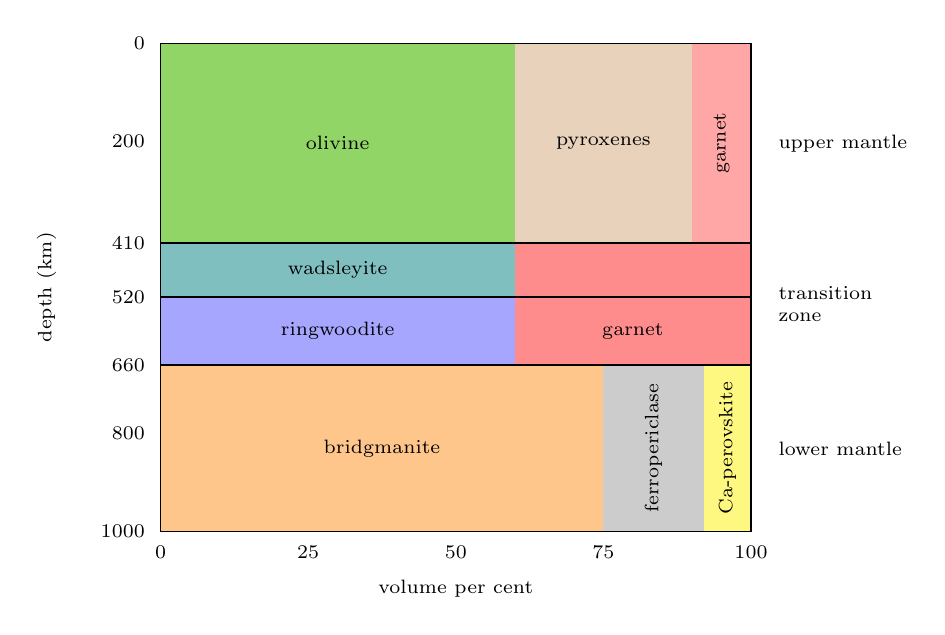
\begin{tikzpicture}[x=0.075mm, y=-0.062mm, font=\scriptsize]
% schematic volume fractions (ledger frost:mantle-transitions, sun:lower-mantle)
\def\W{1000}
% upper mantle 0-410: olivine 60, pyroxenes 30, garnet 10
\fill[green!45!olive!60] (0,0) rectangle (600,410);
\fill[brown!35] (600,0) rectangle (900,410);
\fill[red!35] (900,0) rectangle (1000,410);
% 410-520 wadsleyite 60, garnet 40 ; 520-660 ringwoodite 60, garnet 40
\fill[teal!50] (0,410) rectangle (600,520);
\fill[blue!35] (0,520) rectangle (600,660);
\fill[red!45] (600,410) rectangle (1000,660);
% 660-1000 bridgmanite 75, ferropericlase 17, Ca-perovskite 8
\fill[orange!45] (0,660) rectangle (750,1000);
\fill[gray!40] (750,660) rectangle (920,1000);
\fill[yellow!50] (920,660) rectangle (1000,1000);
\draw (0,0) rectangle (1000,1000);
\foreach \d in {410,520,660} \draw[thick] (0,\d) -- (1000,\d);
\node at (300,205) {olivine};
\node[align=center] at (750,205) {pyroxenes};
\node[rotate=90] at (950,205) {garnet};
\node at (300,465) {wadsleyite};
\node at (300,590) {ringwoodite};
\node[align=center] at (800,590) {garnet};
\node at (375,830) {bridgmanite};
\node[rotate=90, align=center] at (835,830) {ferropericlase};
\node[rotate=90] at (960,830) {Ca-perovskite};
\foreach \d in {0,200,410,520,660,800,1000} \node[anchor=east] at (-10,\d) {\d};
\node[rotate=90, anchor=south] at (-160,500) {depth (km)};
\foreach \p in {0,25,50,75,100} \node[anchor=north] at (\p*10,1010) {\p};
\node[anchor=north] at (500,1080) {volume per cent};
\node[anchor=west, align=left] at (1030,205) {upper mantle};
\node[anchor=west, align=left] at (1030,535) {transition\\zone};
\node[anchor=west, align=left] at (1030,830) {lower mantle};
\end{tikzpicture}

\par\smallskip{\small The \omterm{def:b1:rock-forming-minerals:mineral}{minerals} of a peridotite \omterm{def:b1:layered-earth:layers}{mantle} with depth, as volume
fractions (schematic: the boundaries are drawn sharp, and the fractions are
round values within the ranges quoted in the text). The composition does not
change; the \omterm{def:b1:rock-forming-minerals:mineral}{minerals} do, at about 410, 520 and \qty{660}{km}.}
\end{omfigure}

At the bottom of the \omterm{def:b1:layered-earth:layers}{mantle}, the layer called D$''$ (D double prime, a name
kept from an early model of the Earth) has a velocity gradient different from
the rest of the lower \omterm{def:b1:layered-earth:layers}{mantle}; PREM gives it the lowest \qty{150}{km} of the
\omterm{def:b1:layered-earth:layers}{mantle}. It is seismically heterogeneous: patches of very low speed, steep
gradients, reflectors. It is thought to be a boundary layer between the hot
core and the \omterm{def:b1:layered-earth:layers}{mantle}, and perhaps a graveyard of old slabs.
% ledger: prem:dpp

\section{The core}

The core is mostly iron. Its density, its speeds and its ability to generate a
magnetic field all point to a metal, and iron is by far the most abundant
element dense enough among those that the meteorites and the Sun show to be
common. Nickel, abundant in iron meteorites, accompanies it. But the core is
not pure iron--nickel.
\begin{itemize}
  \item The core is \qtyrange{5}{10}{\percent} less dense than pure iron would
        be at the same pressure and temperature: it must contain light
        elements, among which silicon, sulfur, carbon, oxygen and hydrogen are
        the candidates.
  \item The density jumps by about \qty{4.5}{\percent} at the \omterm{def:b1:layered-earth:discontinuity}{inner-core
        boundary}, too much for the freezing of one and the same metal: the
        \omterm{def:b1:layered-earth:layers}{inner core} holds light elements too, but fewer, a few per cent
        against \qtyrange{5}{10}{\percent} in the liquid.
\end{itemize}
% ledger: badro:core
The difference has a consequence. As the Earth cools --- its \omterm{def:b1:layered-earth:layers}{mantle} by about
\qty{100}{\degreeCelsius} per billion years at present --- the liquid of the core
freezes onto the \omterm{def:b1:layered-earth:layers}{inner core}, which grows, and
% ledger: bellini:cooling
freezing leaves most of the light elements in the liquid. The light liquid
released at the bottom of the \omterm{def:b1:layered-earth:layers}{outer core} rises, and this buoyancy is thought
to help stir the \omterm{def:b1:layered-earth:layers}{outer core} and drive the dynamo that makes the Earth's
magnetic field.

\section{Mechanical layers: lithosphere and asthenosphere}

The layers above are defined by composition and phase: \omterm{def:b1:layered-earth:layers}{crust} and \omterm{def:b1:layered-earth:layers}{mantle} are
different rocks, outer and \omterm{def:b1:layered-earth:layers}{inner core} different states. Plate tectonics needs a
different division, by strength, which cuts across the first one.

\begin{definition}[Lithosphere, asthenosphere, low-velocity zone]
\label{def:b1:layered-earth:lithosphere}
The \emph{lithosphere}\index{lithosphere} is the rigid outer shell of the
Earth, the \omterm{def:b1:layered-earth:layers}{crust} and the uppermost \omterm{def:b1:layered-earth:layers}{mantle}, which behaves as a strong layer
over geological times and is divided into plates. The
\emph{asthenosphere}\index{asthenosphere} is the weaker layer of the upper
\omterm{def:b1:layered-earth:layers}{mantle} below it, which deforms by slow flow and lets the plates move. The
\emph{low-velocity zone}\index{low-velocity zone} is the depth range below the
lithosphere where the seismic speeds, S speeds especially, are lower than just
above and below.
\end{definition}

The \omterm{def:b1:layered-earth:lithosphere}{lithosphere} is not a rock but a temperature range: \omterm{def:b1:layered-earth:layers}{mantle} peridotite is
strong where it is cold and creeps where it is hot, and its base is roughly an
isotherm. It is thin under ridges, where hot \omterm{def:b1:layered-earth:layers}{mantle} rises, about
\qty{140}{km} thick under the oldest ocean floor, and \qtyrange{40}{280}{km}
thick under continents, the thickest under old cratons; the top of the
\omterm{def:b1:layered-earth:lithosphere}{asthenosphere} lies at about \qtyrange{80}{200}{km}. Seismically, the
\omterm{def:b1:layered-earth:lithosphere}{asthenosphere} shows as the \omterm{def:b1:layered-earth:lithosphere}{low-velocity zone}, close to its melting conditions:
in PREM the S speed decreases slightly from the \omterm{def:b1:layered-earth:discontinuity}{Moho} down to \qty{220}{km},
where it jumps up again. How strength depends on temperature, and why it does
so, is the subject of \cref{ch:b1:stress-strain-rheology}.

\begin{inthefield}[A seismic station]
\begin{minipage}[t]{0.55\linewidth}\vspace{0pt}
The travel times on which reference models rest come from permanent
stations. A broadband seismometer, which records ground motions from
hundredths of a second to hours in period, sits on a concrete pier set on bare
rock and isolated from the floor of the vault, under a cover that keeps its
temperature steady: a change of a fraction of a degree, a draught or a passing
lorry would show on the record. The data logger stamps every sample with time
from satellites, and the records stream to data centres that share them
openly. Networks of such stations locate and time every large earthquake; arrival times picked on their records were
inverted for the speeds at each depth.
\end{minipage}\hfill
\begin{minipage}[t]{0.42\linewidth}\vspace{0pt}
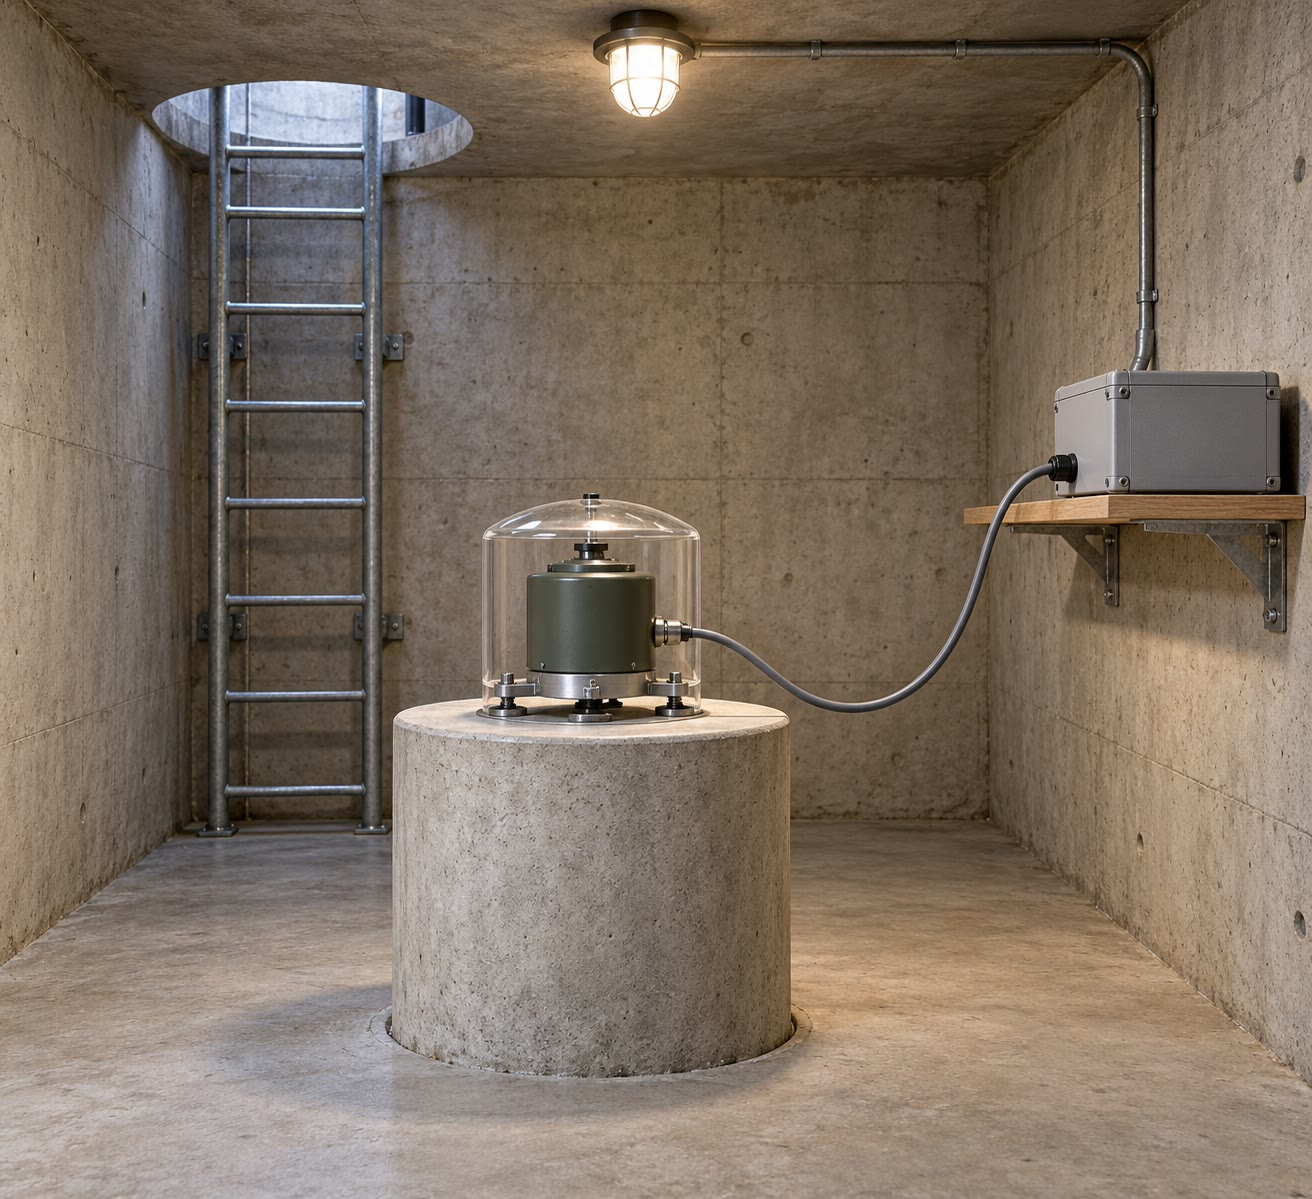
\includegraphics[width=\linewidth]{images/book3/ai/b1-seismometer-vault.jpg}

{\scriptsize A broadband seismometer on its pier in an underground vault, with
the data logger on the wall (AI-generated illustration).}
\end{minipage}
\end{inthefield}

\section{Exercises}

\begin{exercise}[$\star$]\label{exo:b1:layered-earth:1}
With the PREM radii $R = \qty{6371}{km}$, $r_{\text{CMB}} = \qty{3480}{km}$ and
$r_{\text{ICB}} = \qty{1221.5}{km}$, compute the fractions of the Earth's
volume occupied by the core and by the \omterm{def:b1:layered-earth:layers}{inner core}.
% ledger: prem:cmb, prem:icb
\end{exercise}

\begin{exercise}[$\star$]\label{exo:b1:layered-earth:2}
Just above the \omterm{def:b1:layered-earth:discontinuity}{core--mantle boundary} PREM gives $v_P = \qty{13.7166}{km.s^{-1}}$,
$v_S = \qty{7.26466}{km.s^{-1}}$, $\rho = \qty{5.56645}{g.cm^{-3}}$; just below,
$v_P = \qty{8.06482}{km.s^{-1}}$, $v_S = 0$, $\rho = \qty{9.90349}{g.cm^{-3}}$.
Compute the \omterm{def:b1:layered-earth:seismic-parameter}{seismic parameter} and the bulk modulus on each side (in GPa). What
changes most across the boundary?
% ledger: data:prem, prem:cmb
\end{exercise}

\begin{exercise}[$\star$]\label{exo:b1:layered-earth:3}
A \omterm{def:b1:layered-earth:layers}{crust} \qty{30}{km} thick, at \qty{6.2}{km.s^{-1}}, rests on a \omterm{def:b1:layered-earth:layers}{mantle} at
\qty{8.1}{km.s^{-1}}. Compute the critical angle, the critical distance and the
\omterm{def:b1:layered-earth:head-wave}{crossover distance}.
\end{exercise}

\begin{exercise}[$\star$]\label{exo:b1:layered-earth:4}
The core's mass is \qty{1.94e24}{kg} and its radius \qty{3480}{km}. Compute
the gravity at the \omterm{def:b1:layered-earth:discontinuity}{core--mantle boundary} and compare it with the surface
gravity, \qty{9.82}{m.s^{-2}}. Why is it larger?
\end{exercise}

\begin{exercise}[$\star\star$]\label{exo:b1:layered-earth:5}
On a refraction profile the first arrivals are at \qty{10.0}{s} at
\qty{60}{km}, and at \qty{33.3}{s} at \qty{200}{km} and \qty{45.8}{s} at
\qty{300}{km}; the line through the first point passes through the origin.
Find $v_1$, $v_2$, the intercept time and the depth of the boundary, and check
the result with the \omterm{def:b1:layered-earth:head-wave}{crossover distance}.
\end{exercise}

\begin{exercise}[$\star\star$]\label{exo:b1:layered-earth:6}
Show that a uniform sphere has $I = 0.4\,MR^2$. Then compute the mass and the
factor $I/MR^2$ of a two-layer Earth: a core of radius \qty{3480}{km} and
density \qty{11.0}{g.cm^{-3}} in a \omterm{def:b1:layered-earth:layers}{mantle} of density \qty{4.45}{g.cm^{-3}},
with $R = \qty{6371}{km}$. Compare with \num{5.972e24} kg and $0.3308$.
\end{exercise}

\begin{exercise}[$\star\star$]\label{exo:b1:layered-earth:7}
At \qty{1471}{km} depth PREM gives $v_P = \qty{12.16}{km.s^{-1}}$,
$v_S = \qty{6.673}{km.s^{-1}}$, $\rho = \qty{4.86}{g.cm^{-3}}$, and the gravity
is \qty{9.9}{m.s^{-2}}. Compute the density gradient given by the
Adams--Williamson equation, in \unit{g.cm^{-3}} per \qty{1000}{km}, and compare
with PREM's densities, \num{4.844} at \qty{1471}{km} and \num{5.357} at
\qty{2471}{km}.
% ledger: data:prem
\end{exercise}

\begin{exercise}[$\star\star$]\label{exo:b1:layered-earth:8}
Estimate the pressure at \qty{670}{km} depth from a mean density of
\qty{3.57}{g.cm^{-3}} and a gravity of \qty{9.9}{m.s^{-2}}. Which \omterm{def:b1:rock-forming-minerals:mineral}{mineral}
change is expected there?
% ledger: frost:mantle-transitions
\end{exercise}

\begin{exercise}[$\star\star$]\label{exo:b1:layered-earth:9}
PREM's mean density of the \omterm{def:b1:layered-earth:layers}{outer core} is \qty{10.90}{g.cm^{-3}}; at the
\omterm{def:b1:layered-earth:discontinuity}{inner-core boundary} its density is \qty{12.166}{g.cm^{-3}} above and
\qty{12.764}{g.cm^{-3}} below. (a)~If iron at the same conditions is
\qtyrange{5}{10}{\percent} denser than the \omterm{def:b1:layered-earth:layers}{outer core}, what range of densities
does that give for liquid iron there? (b)~Compute the density jump at the
\omterm{def:b1:layered-earth:discontinuity}{inner-core boundary} in per cent, and compare it with the \qty{4.5}{\percent}
of recent studies. (c)~What does a jump larger than freezing alone would give
say about the light elements?
% ledger: badro:core, prem:icb
\end{exercise}

\begin{exercise}[$\star\star\star$]\label{exo:b1:layered-earth:10}
Show that the reflected-wave time $t_r(x) = \sqrt{x^2 + 4h^2}/v_1$ and the
head-wave time of \cref{thm:b1:layered-earth:two-layer} are equal, and have
equal slopes, at $x = 2h\tan i_c$, and that $t_r > t_{\text{head}}$ beyond it.
Interpret.
\end{exercise}

\begin{exercise}[$\star\star\star$]\label{exo:b1:layered-earth:11}
For an Earth of uniform density $\rho$, show that $g(r) = \tfrac43\pi G\rho r$
and $P(r) = \tfrac23\pi G\rho^2(R^2 - r^2)$. Compute the central pressure with
$\rho = \qty{5513}{kg.m^{-3}}$ and $R = \qty{6371}{km}$, and compare with PREM's
\qty{363.85}{GPa}.
% ledger: earth:density, prem:centre
\end{exercise}

\begin{exercise}[$\star\star\star$]\label{exo:b1:layered-earth:12}
Show that if $g/\Phi$ is constant through a layer, the Adams--Williamson
equation gives $\rho = \rho_0\exp\bigl(g(z - z_0)/\Phi\bigr)$ with depth $z$.
Apply it to the \omterm{def:b1:layered-earth:layers}{outer core}, from \qty{2891}{km} ($\rho_0 =
\qty{9.90}{g.cm^{-3}}$) to \qty{5149.5}{km}, with mean values
$g = \qty{7.9}{m.s^{-2}}$ and $\Phi = \qty{87}{km^2.s^{-2}}$; compare with
PREM's \qty{12.17}{g.cm^{-3}} at the \omterm{def:b1:layered-earth:discontinuity}{inner-core boundary}.
% ledger: prem:icb
\end{exercise}

\section{Problem: Weighing the Earth's shells}

\begin{problem}[{Weekend problem --- volumes, masses and moment of inertia of a
four-shell Earth built from PREM, compared with the measured mass and moment of
inertia; gravity and pressure deep inside}]
\label{pb:b1:layered-earth:1}
% values: calc/ch09.py; mean densities rounded from figdata prem_profiles (values part)
% ledger: data:prem, prem:constraints, prem:centre, prem:cmb, earth:mass, earth:MoI, const:G
The Earth is cut into four shells at the radii of PREM, and each is given its
mean density in PREM, rounded:
\begin{center}
\small
\begin{tabular}{lccc}
\hline
shell & from (km) & to (km) & mean density (\unit{g.cm^{-3}}) \\
\hline
\omterm{def:b1:layered-earth:layers}{crust}, upper \omterm{def:b1:layered-earth:layers}{mantle} and transition zone & 5701 & 6371 & 3.57 \\
lower \omterm{def:b1:layered-earth:layers}{mantle} & 3480 & 5701 & 4.90 \\
\omterm{def:b1:layered-earth:layers}{outer core} & 1221.5 & 3480 & 10.90 \\
\omterm{def:b1:layered-earth:layers}{inner core} & 0 & 1221.5 & 12.89 \\
\hline
\end{tabular}
\end{center}
Use $G = \qty{6.674e-11}{m^3.kg^{-1}.s^{-2}}$. The measured mass of the Earth
is \qty{5.972e24}{kg} and its \omterm{def:b1:comparative-planetology:moi}{moment-of-inertia factor} $I/MR^2 = 0.3308$.

\medskip
\noindent\textbf{Part I --- Volumes.}
\begin{enumerate}
  \item Compute the volume of the Earth.
  \item Compute the volume of each shell.
  \item What fraction of the volume does each shell occupy? Which shell is
        the largest?
  \item What fraction of the volume is core?
\end{enumerate}

\noindent\textbf{Part II --- Masses.}
\begin{enumerate}[resume]
  \item Compute the mass of each shell.
  \item Add them, and compare the total with the measured mass.
  \item Deduce the mean density of the model Earth.
  \item What fraction of the mass is in the \omterm{def:b1:layered-earth:layers}{inner core}?
  \item What fraction of the mass is in the \omterm{def:b1:layered-earth:layers}{mantle} and \omterm{def:b1:layered-earth:layers}{crust} together?
  \item Compare the core's share of the volume and of the mass, and explain.
\end{enumerate}

\noindent\textbf{Part III --- Moment of inertia.}
\begin{enumerate}[resume]
  \item Show from \cref{prop:b1:layered-earth:integrals} that a uniform shell
        between $r_1$ and $r_2$ has $I = \tfrac{8\pi}{15}\rho\,(r_2^5 - r_1^5)$.
  \item Compute the moment of inertia of each shell.
  \item Which shell contributes most, and why does the \omterm{def:b1:layered-earth:layers}{inner core} contribute
        almost nothing?
  \item Add them and compute $I/MR^2$ for the model.
  \item Compare with $0.3308$ and with the $0.4$ of a uniform sphere.
  \item Inside each real shell the density increases with depth. Does that
        explain why the model's factor is too high? Explain.
\end{enumerate}

\noindent\textbf{Part IV --- Gravity and pressure.}
\begin{enumerate}[resume]
  \item Compute the gravity at the surface of the model.
  \item Compute the gravity at the \omterm{def:b1:layered-earth:discontinuity}{core--mantle boundary}.
  \item Compute the mean density of the \omterm{def:b1:layered-earth:layers}{mantle} and \omterm{def:b1:layered-earth:layers}{crust} together.
  \item Gravity in the \omterm{def:b1:layered-earth:layers}{mantle} stays close to \qty{10}{m.s^{-2}}. Estimate the
        pressure at the \omterm{def:b1:layered-earth:discontinuity}{core--mantle boundary}, and compare with PREM's
        \qty{135.75}{GPa}.
  \item Compute the mean density of the core, and the pressure increase from
        the \omterm{def:b1:layered-earth:discontinuity}{core--mantle boundary} to the centre in a uniform core,
        $\tfrac23\pi G\rho_c^2 r_c^2$ (\cref{exo:b1:layered-earth:11} applied to the core alone).
  \item Add the two to estimate the central pressure, and compare with PREM's
        \qty{363.85}{GPa}. Why is the estimate too low?
  \item Which of the model's numbers are checked against a measurement, and
        which only against PREM itself?
  \item What fraction of the Earth's mass lies in the core?
\end{enumerate}
\end{problem}
